% !TeX root = RJwrapper.tex
\title{Current status and propsects of R-packages for the design of
experiments}
\author{by Emi Tanaka}

\maketitle

\abstract{%
Re-running an experiment is generally costly and in some cases
impossible due to limited resources, so the design of experiment plays a
critical role in increasing the quality of experimental data. In this
article I describe the current state of the R-packages for the design of
experiments through textual analysis and download trends. I discuss also
the software design of widely utilised R packages in the field of
experimental design and conclude with discussion of some future
prospects for the field.
}

\hypertarget{introduction}{%
\section{Introduction}\label{introduction}}

The critical role of data collection is well captured in the expression
``garbage in, garbage out'' -- in other words, if the collected data is
rubbish then no analysis, however complex it may be, can make something
out of it. Methods for data collection can be dichotomised by the type
of data collected -- namely, experimental or observational -- or
alternatively, categorised into experimental design or survey design.
Survey designs often, although not always, aim to collect observational
data whilst experimental designs exclusively center on experimental
data. This dichotomisation, to a great extent, is seen in CRAN task
views where R-packages in experimental design are in
\ctv{ExperimentalDesign} and R-packages in survey designs are in
\ctv{OfficialStatistics}.

In the CRAN task view of \ctv{ExperimentalDesign}, there are 113 R
packages for experimental design and analysis of data from experiments,
henceforth referred to as ``DoE packages'' in this paper. The sheer
quantity and variation in the output experimental design in the
R-packages are arguably unmatched with any other programming languages,
e.g.~in Python \citep{python}, only a handful of libraries that generate
design of experiment exist (namely \texttt{pyDOE}, \texttt{pyDOE2},
\texttt{dexpy}, \texttt{experimenter} and \texttt{GPdoemd}) with limited
outputs.

\hypertarget{explorative-analysis}{%
\section{Explorative Analysis}\label{explorative-analysis}}

\begin{Schunk}
\begin{figure}[htbp]

{\centering 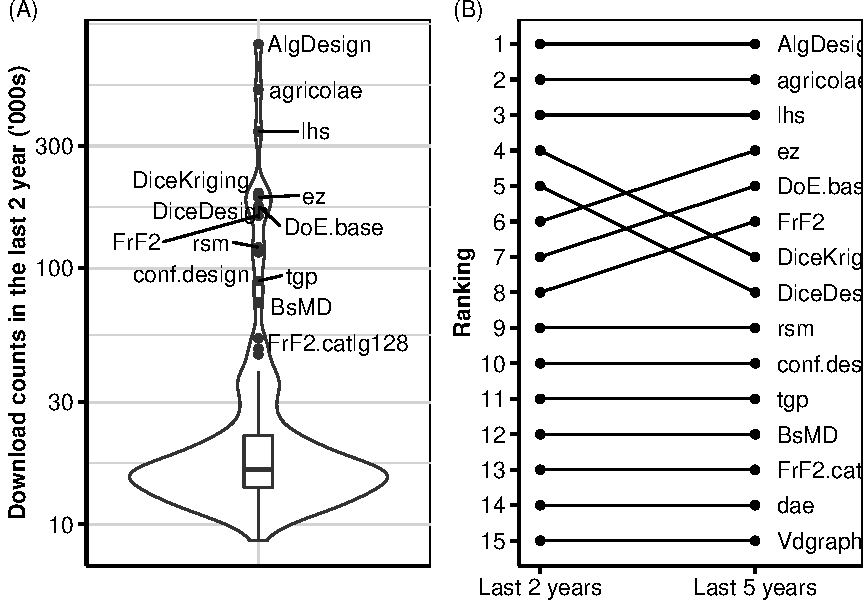
\includegraphics{paper_files/figure-latex/dlplots-1} 

}

\caption[The above graph shows the total download counts from 2019-03-06 to 2021-03-04 of DoE packages]{The above graph shows the total download counts from 2019-03-06 to 2021-03-04 of DoE packages.}\label{fig:dlplots}
\end{figure}
\end{Schunk}

\begin{itemize}
\tightlist
\item
  Not much difference between title and description.
\item
  Just go with description and combine bi \& tri.
\end{itemize}

\begin{Schunk}


\begin{center}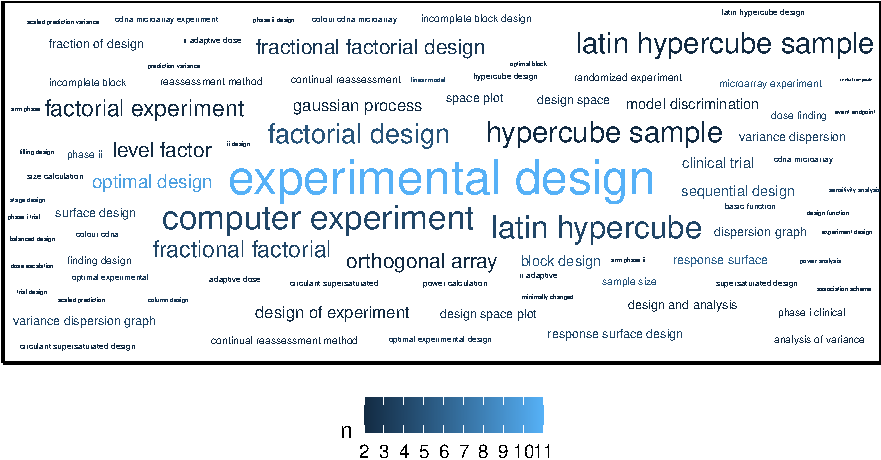
\includegraphics{paper_files/figure-latex/wordcloud-1} \end{center}

\end{Schunk}

\hypertarget{what-are-the-common-types-of-experimental-designs}{%
\subsection{What are the common types of experimental
designs?}\label{what-are-the-common-types-of-experimental-designs}}

\hypertarget{how-do-packages-interplay-with-each-other}{%
\subsection{How do packages interplay with each
other?}\label{how-do-packages-interplay-with-each-other}}

\hypertarget{which-packages-are-widely-utilised}{%
\subsection{Which packages are widely
utilised?}\label{which-packages-are-widely-utilised}}

\hypertarget{software-design}{%
\section{Software Design}\label{software-design}}

\hypertarget{propsects-and-discussion}{%
\section{Propsects and Discussion}\label{propsects-and-discussion}}

\newpage

\begin{table}[h] \centering  
\begin{tabular}[t]{lr}
\toprule
word & n\\
\midrule
optimal design & 10\\
experimental design & 8\\
clinical trial & 5\\
dose finding & 5\\
sequential design & 5\\
block design & 4\\
microarray experiment & 4\\
response surface & 4\\
\bottomrule
\end{tabular} \hspace{1cm} \centering  
\begin{tabular}[t]{lr}
\toprule
word & n\\
\midrule
experimental design & 11\\
optimal design & 10\\
package provide & 7\\
graphical user & 6\\
response surface & 6\\
user interface & 6\\
block design & 5\\
contour plot & 5\\
design based & 5\\
effect model & 5\\
factorial design & 5\\
microarray experiment & 5\\
mixed effect & 5\\
provide function & 5\\
sample size & 5\\
sequential design & 5\\
\bottomrule
\end{tabular} \caption{My tables} \end{table}

\CRANpkg{agricolae}

\hypertarget{helping-info-to-get-started}{%
\subsection{Helping info to get
started}\label{helping-info-to-get-started}}

Introductory section which may include references in parentheses
\citep{R}, or cite a reference such as \citet{R} in the text.

\hypertarget{section-title-in-sentence-case}{%
\subsection{Section title in sentence
case}\label{section-title-in-sentence-case}}

Let's check fi this works Figure @ref(fig:Rlogo).

This section may contain a figure such as Figure \ref{fig:Rlogo}.

\hypertarget{summary}{%
\subsection{Summary}\label{summary}}

This file is only a basic article template. For full details of
\emph{The R Journal} style and information on how to prepare your
article for submission, see the
\href{https://journal.r-project.org/share/author-guide.pdf}{Instructions
for Authors}.

\hypertarget{about-this-format-and-the-r-journal-requirements}{%
\subsubsection{About this format and the R Journal
requirements}\label{about-this-format-and-the-r-journal-requirements}}

\texttt{rticles::rjournal\_article} will help you build the correct
files requirements:

\begin{itemize}
\tightlist
\item
  A R file will be generated automatically using \texttt{knitr::purl} -
  see \url{https://bookdown.org/yihui/rmarkdown-cookbook/purl.html} for
  more information.
\item
  A tex file will be generated from this Rmd file and correctly included
  in \texttt{RJwapper.tex} as expected to build \texttt{RJwrapper.pdf}.
\item
  All figure files will be kept in the default rmarkdown
  \texttt{*\_files} folder. This happens because
  \texttt{keep\_tex\ =\ TRUE} by default in
  \texttt{rticles::rjournal\_article}
\item
  Only the bib filename is to modifed. An example bib file is included
  in the template (\texttt{RJreferences.bib}) and you will have to name
  your bib file as the tex, R, and pdf files.
\end{itemize}

\bibliography{paper.bib}

\address{%
Emi Tanaka\\
Monash University\\%
Monash University\\ Clayton campus, VIC 3800, Australia\\
%
\url{http://emitanaka.org/}%
\\\textit{ORCiD: \href{https://orcid.org/0000-0002-1455-259X}{0000-0002-1455-259X}}%
\\\href{mailto:emi.tanaka@monash.edu}{\nolinkurl{emi.tanaka@monash.edu}}
}
